%package list
\documentclass{article}
\usepackage[top=3cm, bottom=3cm, outer=3cm, inner=3cm]{geometry}
\usepackage{multicol}
\usepackage{graphicx}
\usepackage{url}
%\usepackage{cite}
\usepackage{hyperref}
\usepackage{array}
%\usepackage{multicol}
\newcolumntype{x}[1]{>{\centering\arraybackslash\hspace{0pt}}p{#1}}
\usepackage{natbib}
\usepackage{pdfpages}
\usepackage{multirow}
\usepackage[normalem]{ulem}
\useunder{\uline}{\ul}{}
\usepackage{svg}
\usepackage{xcolor}
\usepackage{listings}
\lstdefinestyle{ascii-tree}{
    literate={├}{|}1 {─}{--}1 {└}{+}1 
  }
\lstset{basicstyle=\ttfamily,
  showstringspaces=false,
  commentstyle=\color{red},
  keywordstyle=\color{blue}
}
%\usepackage{booktabs}
\usepackage{caption}
\usepackage{subcaption}
\usepackage{float}
\usepackage{array}

\newcolumntype{M}[1]{>{\centering\arraybackslash}m{#1}}
\newcolumntype{N}{@{}m{0pt}@{}}


%%%%%%%%%%%%%%%%%%%%%%%%%%%%%%%%%%%%%%%%%%%%%%%%%%%%%%%%%%%%%%%%%%%%%%%%%%%%
%%%%%%%%%%%%%%%%%%%%%%%%%%%%%%%%%%%%%%%%%%%%%%%%%%%%%%%%%%%%%%%%%%%%%%%%%%%%
\newcommand{\itemEmail}{fayamamani@unsa.edu.pe}
\newcommand{\itemStudent}{Francis Willian Ayamamani Añasco}
\newcommand{\itemCourse}{Programación Web 2}
\newcommand{\itemCourseCode}{GUIA-PRLD-001}
\newcommand{\itemSemester}{I}
\newcommand{\itemUniversity}{Universidad Nacional de San Agustín de Arequipa}
\newcommand{\itemFaculty}{Facultad de Ingeniería de Producción y Servicios}
\newcommand{\itemDepartment}{Departamento Académico de Ingeniería de Sistemas e Informática}
\newcommand{\itemSchool}{Escuela Profesional de Ingeniería de Sistemas}
\newcommand{\itemAcademic}{2023 - A}
\newcommand{\itemInput}{Del 5 Junio 2023}
\newcommand{\itemOutput}{Al 5 Junio 2023}
\newcommand{\itemPracticeNumber}{02}
\newcommand{\itemTheme}{JavaScript}
%%%%%%%%%%%%%%%%%%%%%%%%%%%%%%%%%%%%%%%%%%%%%%%%%%%%%%%%%%%%%%%%%%%%%%%%%%%%
%%%%%%%%%%%%%%%%%%%%%%%%%%%%%%%%%%%%%%%%%%%%%%%%%%%%%%%%%%%%%%%%%%%%%%%%%%%%

\usepackage[english,spanish]{babel}
\usepackage[utf8]{inputenc}
\AtBeginDocument{\selectlanguage{spanish}}
\renewcommand{\figurename}{Figura}
\renewcommand{\refname}{Referencias}
\renewcommand{\tablename}{Tabla} %esto no funciona cuando se usa babel
\AtBeginDocument{%
	\renewcommand\tablename{Tabla}
}

\usepackage{fancyhdr}
\pagestyle{fancy}
\fancyhf{}
\setlength{\headheight}{30pt}
\renewcommand{\headrulewidth}{1pt}
\renewcommand{\footrulewidth}{1pt}
\fancyhead[L]{\raisebox{-0.2\height}{
\includegraphics[width=3cm]{img/logo_episunsa.png}}}
\fancyhead[C]{\fontsize{7}{7}\selectfont	\itemUniversity \\ \itemFaculty \\ \itemDepartment \\ \itemSchool \\ \textbf{\itemCourse}}
\fancyhead[R]{\raisebox{-0.2\height}{
\includegraphics[width=1.2cm]{img/logo_abet}}}
\fancyfoot[L]{Estudiante Francis Ayamamani Añasco}
\fancyfoot[C]{\itemCourse}
\fancyfoot[R]{Página \thepage}

% para el codigo fuente
\usepackage{listings}
\usepackage{color, colortbl}
\definecolor{dkgreen}{rgb}{0,0.6,0}
\definecolor{gray}{rgb}{0.5,0.5,0.5}
\definecolor{mauve}{rgb}{0.58,0,0.82}
\definecolor{codebackground}{rgb}{0.95, 0.95, 0.92}
\definecolor{tablebackground}{rgb}{0.8, 0, 0}

\lstset{frame=tb,
	language=bash,
	aboveskip=3mm,
	belowskip=3mm,
	showstringspaces=false,
	columns=flexible,
	basicstyle={\small\ttfamily},
	numbers=none,
	numberstyle=\tiny\color{gray},
	keywordstyle=\color{blue},
	commentstyle=\color{dkgreen},
	stringstyle=\color{mauve},
	breaklines=true,
	breakatwhitespace=true,
	tabsize=3,
	backgroundcolor= \color{codebackground},
}

\begin{document}
	
	\vspace*{10px}
	
	\begin{center}	
		\fontsize{17}{17} \textbf{ Informe de Laboratorio \itemPracticeNumber}
	\end{center}
	\centerline{\textbf{\Large Tema: \itemTheme}}
	%\vspace*{0.5cm}	

	\begin{flushright}
		\begin{tabular}{|M{2.5cm}|N|}
			\hline 
			\rowcolor{tablebackground}
			\color{white} \textbf{Nota}  \\
			\hline 
			     \\[30pt]
			\hline 			
		\end{tabular}
	\end{flushright}	

	\begin{table}[H]
		\begin{tabular}{|x{4.7cm}|x{4.8cm}|x{4.8cm}|}
			\hline 
			\rowcolor{tablebackground}
			\color{white} \textbf{Estudiante} & \color{white}\textbf{Escuela}  & \color{white}\textbf{Asignatura}   \\
			\hline 
			{\itemStudent \par \itemEmail} & \itemSchool & {\itemCourse \par Semestre: \itemSemester \par Código: \itemCourseCode}     \\
			\hline 			
		\end{tabular}
	\end{table}		
	
	\begin{table}[H]
		\begin{tabular}{|x{4.7cm}|x{4.8cm}|x{4.8cm}|}
			\hline 
			\rowcolor{tablebackground}
			\color{white}\textbf{Laboratorio} & \color{white}\textbf{Tema}  & \color{white}\textbf{Duración}   \\
			\hline 
			\itemPracticeNumber & \itemTheme & 04 horas   \\
			\hline 
		\end{tabular}
	\end{table}
	
	\begin{table}[H]
		\begin{tabular}{|x{4.7cm}|x{4.8cm}|x{4.8cm}|}
			\hline 
			\rowcolor{tablebackground}
			\color{white}\textbf{Semestre académico} & \color{white}\textbf{Fecha de inicio}  & \color{white}\textbf{Fecha de entrega}   \\
			\hline 
			\itemAcademic & \itemInput &  \itemOutput  \\
			\hline 
		\end{tabular}
	\end{table}
	
	\section{Tarea}
	\begin{itemize}		
		\item Ejercicio 01: Utilizando JavaScript, genere un teclado aleatorio para Banca por Internet.
Funcionalidad: Los números presionados generan una clave.
        \begin{figure}[H]
		\centering
		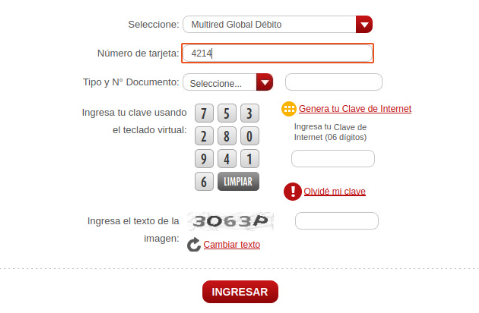
\includegraphics[width=0.8\textwidth,keepaspectratio]{img/Banco.png}
		%\includesvg{img/automata.svg}
		%\label{img:mot2}
		%\caption{Product backlog.}
	   \end{figure}
        \item Ejercicio 02: Utilizando JavaScript, genere una calculadora como la siguiente imagen. 
Cada vez que se presiona ENTER se guardan los datos involucrados en un pila.
        \begin{figure}[H]
		\centering
		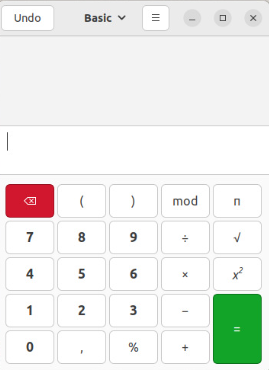
\includegraphics[width=0.8\textwidth,keepaspectratio]{img/Calculadora.png}
		%\includesvg{img/automata.svg}
		%\label{img:mot2}
		%\caption{Product backlog.}
	   \end{figure}
		\end{itemize}
	\section{MARCO CONCEPTUAL}
	\begin{itemize}
		\item Editor Vim
        \begin{itemize}
            \item Vim es un editor de texto muy eficiente para programar en consola que no tiene nada que envidiar a los editores gráficos.
        \end{itemize}
        \item Instalar Vim en
        \begin{itemize}
            \item GNU/Linux
            \begin{itemize}
                \begin{lstlisting}
                    apt-get install vim
                \end{lstlisting}
            \end{itemize}
            \item MS Windows
            \begin{itemize}
                \item Para descarga en sistemas MS Windows \url{https://www.vim.org/download.php}
            \end{itemize}
            \item MacOS
            \begin{itemize}
                \begin{lstlisting}
                    brew install macvim
                \end{lstlisting}
            \end{itemize}
        \end{itemize}
        \item Git
        \begin{itemize}
            \item Git es un sistema de control de versiones creado por Linus Torvalds. Es eficiente, confiable.
        \end{itemize}
        \item Instalar Git
        \begin{itemize}
            \item GNU/Linux
            \begin{itemize}
                \begin{lstlisting}
                apt-get install git    
                \end{lstlisting}
            \end{itemize}
            \item MS Windows
            \begin{itemize}
                \item Para descarga en sistemas MS Windows \url{https://git-scm.com/download/win}
            \end{itemize}
            \item MacOS
            \begin{itemize}
                \item Para descarga en sistemas MacOS \url{https://git-scm.com/download/mac}
                \begin{verbatim}
                    brew install git
                \end{verbatim}
            \end{itemize}
        \end{itemize}
	\end{itemize}
	
	\section{URL de Repositorio Github}
	\begin{itemize}
		\item URL del Repositorio GitHub para clonar o recuperar.
		\item \url{https://github.com/rescobedoq/pw2/tree/main/labs/lab02}
		\item URL para el laboratorio 01 en el Repositorio GitHub.
		\item \url{https://github.com/rescobedoq/pw2/tree/main/labs/lab02}
	\end{itemize}
	
	\section{Resolucion de la tarea}
	
	\subsection{Explicacion del Codigo1}
    \begin{figure}[H]
		\centering
		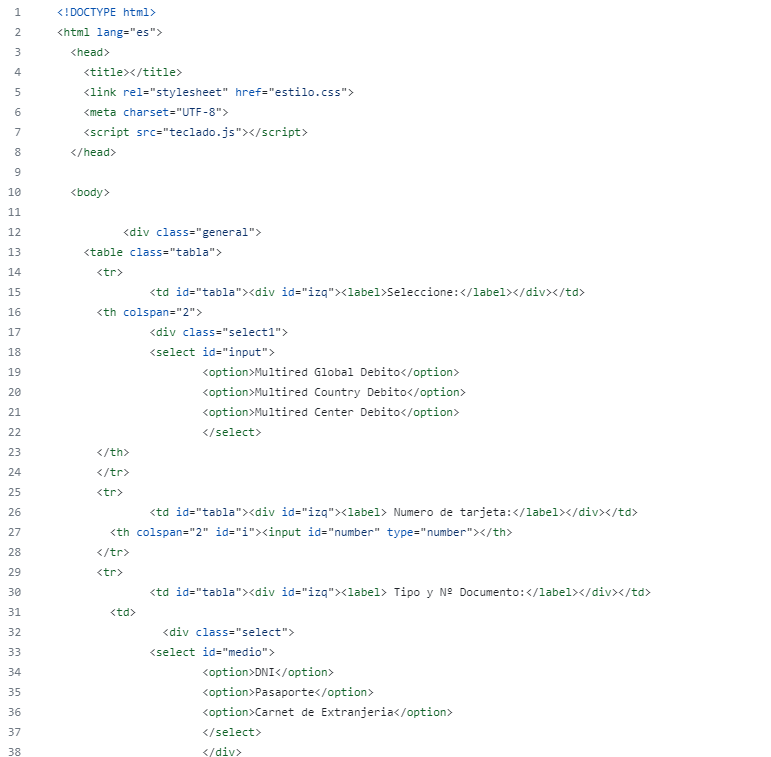
\includegraphics[width=0.8\textwidth,keepaspectratio]{img/parte1.1.png}
		%\includesvg{img/automata.svg}
		%\label{img:mot2}
		%\caption{Product backlog.}
	\end{figure}
 \begin{figure}[H]
		\centering
		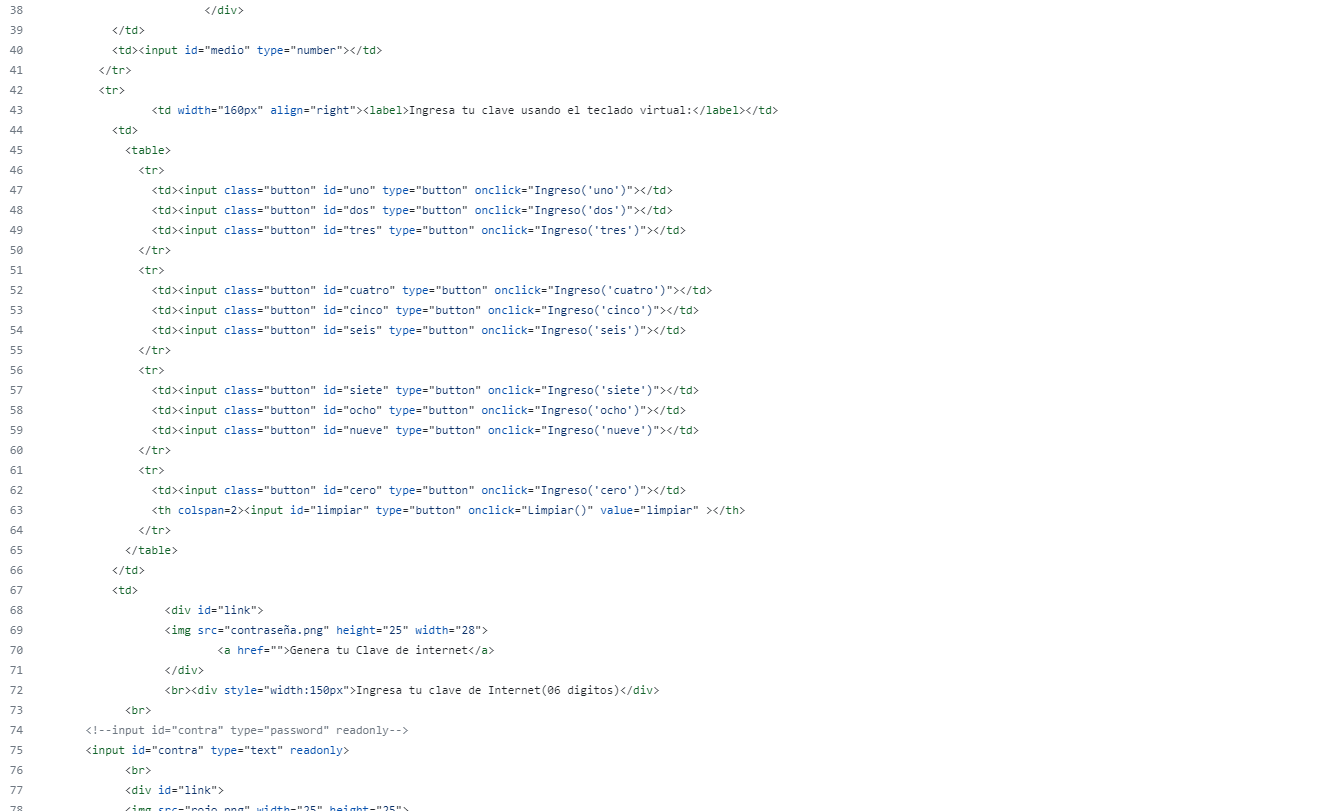
\includegraphics[width=0.8\textwidth,keepaspectratio]{img/parte1.2.png}
		%\includesvg{img/automata.svg}
		%\label{img:mot2}
		%\caption{Product backlog.}
	\end{figure}
 \begin{figure}[H]
		\centering
		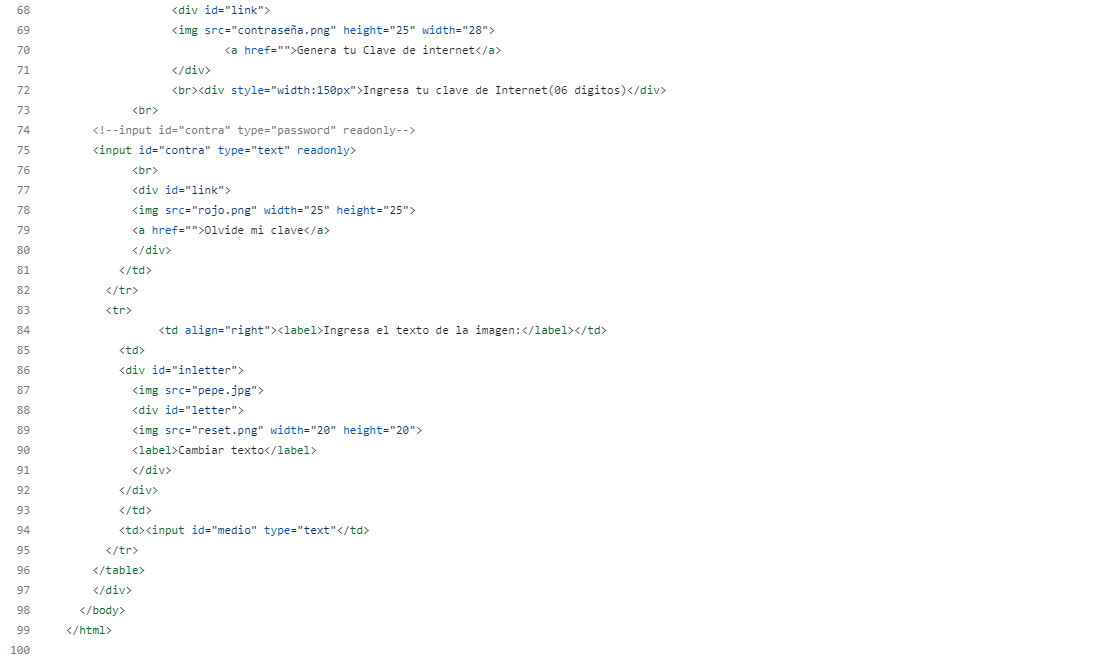
\includegraphics[width=0.8\textwidth,keepaspectratio]{img/parte1.3.png}
		%\includesvg{img/automata.svg}
		%\label{img:mot2}
		%\caption{Product backlog.}
	\end{figure}
	En este archivo cree una estructura html, con etiquetas de input, div, table y entre otros.
 La tabla la utilize para poder simular el div, de cada parte; por lo que entonces, me centre en atributos de cada elemento para acomodar los botones.
 \begin{figure}[H]
		\centering
		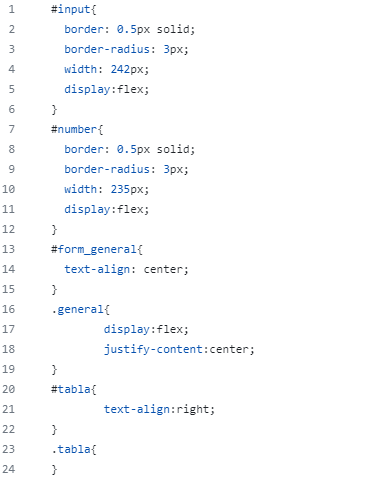
\includegraphics[width=0.8\textwidth,keepaspectratio]{img/style1.png}
		%\includesvg{img/automata.svg}
		%\label{img:mot2}
		%\caption{Product backlog.}
	\end{figure}
 \begin{figure}[H]
		\centering
		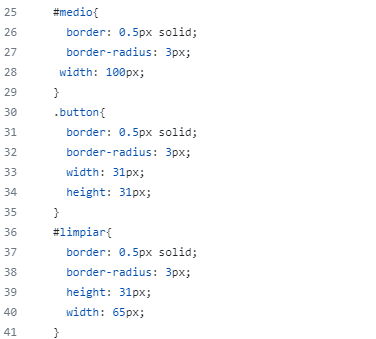
\includegraphics[width=0.8\textwidth,keepaspectratio]{img/style2.png}
		%\includesvg{img/automata.svg}
		%\label{img:mot2}
		%\caption{Product backlog.}
	\end{figure}
 \begin{figure}[H]
		\centering
		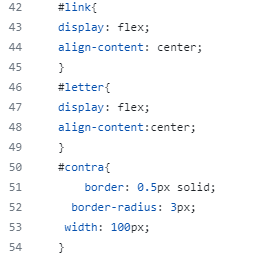
\includegraphics[width=0.8\textwidth,keepaspectratio]{img/style3.png}
		%\includesvg{img/automata.svg}
		%\label{img:mot2}
		%\caption{Product backlog.}
	\end{figure}
 Finalmente el archivo teclado.js, es la programacion, del cambio de valor en el boton del teclado
 \begin{figure}[H]
		\centering
		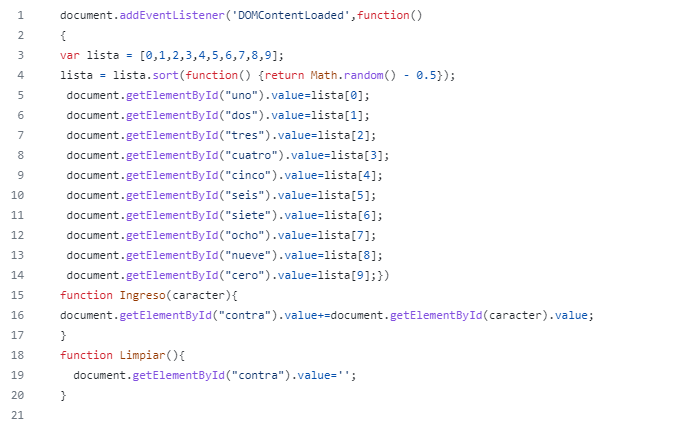
\includegraphics[width=0.8\textwidth,keepaspectratio]{img/teclado.png}
		%\includesvg{img/automata.svg}
		%\label{img:mot2}
		%\caption{Product backlog.}
	\end{figure}
 En estas lineas, genero una variable local, que contenga un array con todos los numeros del teclado, para luego con la funcion list.sort, con la ubicacion generada por la funcion directa de Math.random()-0.5, genera la distribucion del nuevo teclado; finalmente con las lineas de document.getElementById, podemos acceder al elemento button, y cambiar su valor con la funcion value
 \subsection{Explicacion del codigo 2}
    \begin{lstlisting}[language=bash,caption={app.use}][H]
		app.use(express.static('public'));
        app.use(express.urlencoded({extended: true}));
	\end{lstlisting}
    la contante app, en la primera linea establece ala carpeta public como recurso para su ejecucion.Y la siguiente estable el enlace POST.
    \begin{figure}[H]
		\centering
		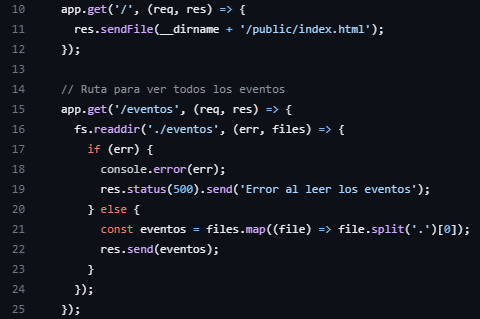
\includegraphics[width=0.8\textwidth,keepaspectratio]{img/indexjs2.png}
		%\includesvg{img/automata.svg}
		%\label{img:mot2}
		%\caption{Product backlog.}
	\end{figure}
    En las lineas 10 a la 12 se hace llamado a la rama principal que hace imprime el index.html
    En las lineas 15 a la 25 nos refrencia en la direccion '/eventos', para imprimir el listado de elementos en el elemento './eventos' que se encuentra como argumento en la funcion de fs.readdir()
    \begin{figure}[H]
		\centering
		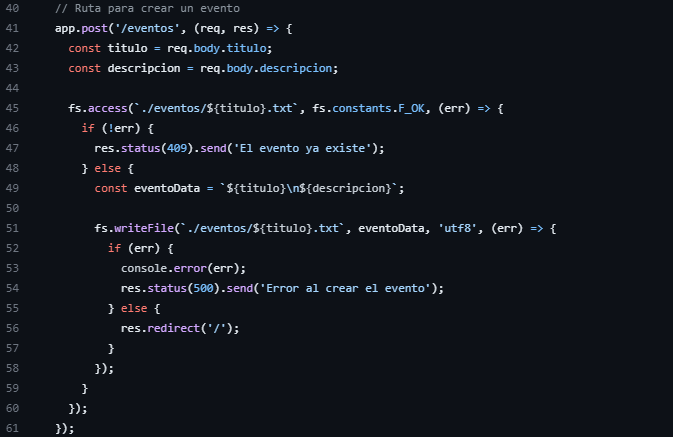
\includegraphics[width=0.8\textwidth,keepaspectratio]{img/indexjs3.png}
		%\includesvg{img/automata.svg}
		%\label{img:mot2}
		%\caption{Product backlog.}
	\end{figure}
    En las lineas 41 a la 43 nos refrencia al metodo POST, crear un archivo en el listado de elementos, definimos una variable como titulo, que es el argumento que nos envian; de igual manera la descripcion.
    (45-61) se ubica en la carpeta de './eventos' para luego entrar en el archivo 'titulo', y verificar su existencia:
    \begin{itemize}
        \item \textbf{TRUE}, le envia el mensaje: "El evento ya existe"
        \item \textbf{FALSE}, concatena el titulo y la descripcion con un salto de linea
        \begin{itemize}
            \item ejecuta la funcion de fs.write, para crear el archivo, agregarle el contenido (Titulo-descripcion)
            \begin{itemize}
                \item \textbf{TRUE}, lo dirige a la rama principal
                \item \textbf{FALSE}, imprime "Error al crear el evento"
            \end{itemize}
        \end{itemize}
    \end{itemize}
    \begin{figure}[H]
		\centering
		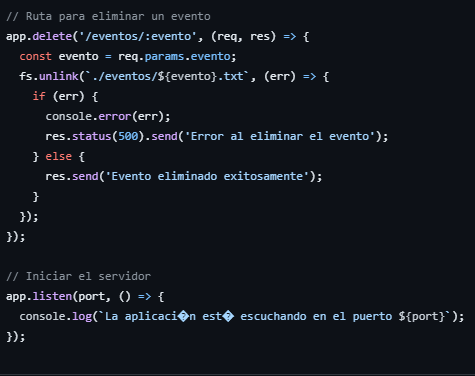
\includegraphics[width=0.8\textwidth,keepaspectratio]{img/indexjs4.png}
		%\includesvg{img/automata.svg}
		%\label{img:mot2}
		%\caption{Product backlog.}
	\end{figure}
    En las lineas 4de app.delete remueve la |ruta de ./eventos/:eventos; siendo ':evento' la variable del archivo, y para ello la definimos esta variable dentro de la funcion, con la constante evento.
    \\Luego la funcion fs.unlink remueve el archivo en la direccion "./eventos/evento.txt"
    \begin{itemize}
        \item \textbf{TRUE}, ejecuta la linea que imprimr "Evento eliminado exitosamente"
        \item \textbf{FALSE}, imprime "Error al eliminar el evento"
    \end{itemize}
    Finalmente la linea conocida para determinar el puerto del servidor y su ejecucion
    \subsection{./public/script.js}
    \begin{figure}[H]
		\centering
		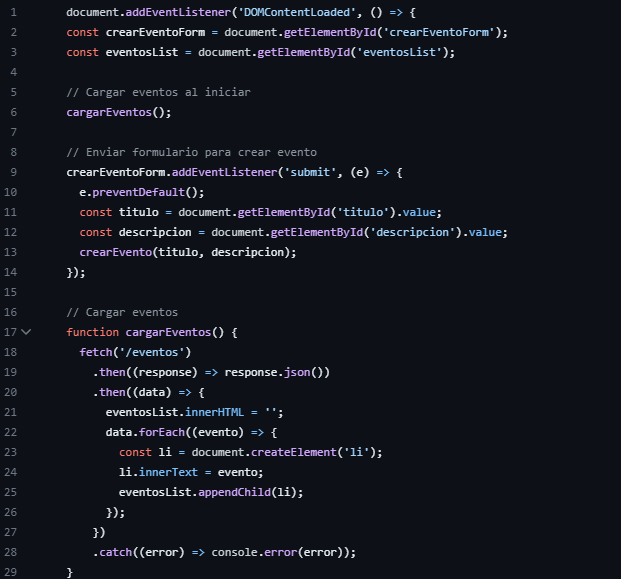
\includegraphics[width=0.8\textwidth,keepaspectratio]{img/script1.png}
		%\includesvg{img/automata.svg}
		%\label{img:mot2}
		%\caption{Product backlog.}
	\end{figure}
 \begin{figure}[H]
		\centering
		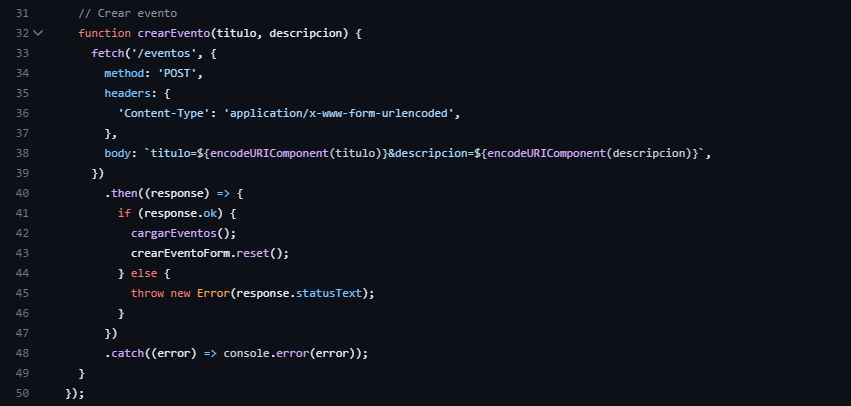
\includegraphics[width=0.8\textwidth,keepaspectratio]{img/script2.png}
		%\includesvg{img/automata.svg}
		%\label{img:mot2}
		%\caption{Product backlog.}
	\end{figure}
    En este archivo declaro las funciones del archivo html para direccionar a una nueva ruta, y de la misma manera vincular las elementos impregnados de una funcion POST
	\subsection{Estructura de laboratorio 02}
	\begin{itemize}	
		\item El contenido que se entrega en este laboratorio es el siguiente:
	\end{itemize}
	
\begin{lstlisting}[style=ascii-tree]
lab2/
|--- LATEX/
    |   |--- main.tex
    |   |--- lab3.pdf
    |   |--- img/
        |   |--- Calculadora.png
        |   |--- indexs1.png
        |   |--- indexs2.png
        |   |--- indexs3.png
        |   |--- indexs4.png
        |   |--- logo_abet.png
        |   |--- logo_episunsa.png
        |   |--- logo_unsa.png
        |   |--- parte1.1.png
        |   |--- parte1.2.png
        |   |--- parte1.3.png
        |   |--- script1.png
        |   |--- script2.png
        |   |--- style1.png
        |   |--- style2.png
        |   |--- style3.png
        |   |--- teclado.png
|--- parte1/
    |   |--- Ejercicio1.html
    |   |--- contraseña.png
    |   |--- estilo.css
    |   |--- pepe.jpg
    |   |--- reset - copia.png
    |   |--- reset.png
    |   |--- rojo.png
    |   |--- teclado.js
|--- parte2/
    |   |--- calculadora.html
    |   |--- funcion.js
    |   |--- style.css
|--- partes_de_prueba/
    |   |--- Ejercicio1.2.html
    |   |--- prototipo de CSS
\end{lstlisting}
\section{Cuestionario}
\begin{itemize}
    \item Pruebe este código de arrayGenerator() en la página https://jslint.com/
    \item Revisar esta discusión en stackoverflow - \url{https://stackoverflow.com/questions/4852017/how-to-initialize-an-arrays-length-in-javascript}
    \begin{itemize}
        \item ¿Cómo se pueden resolver los warnings?
        \\Para resolver los errores y warnings relacionados con la inicialización del tamaño de un array en JavaScript, puedes utilizar la asignación de la propiedad length después de crear un array vacío, o agregar un punto y coma ';' al final de la declaración del array si deseas especificar el tamaño al momento de la inicialización.
        \item ¿Se puede modificar la solución usando map? ¿Cómo?
        Puedo empezar creando una variable que defina el tamaño, luego para rellenar los valores asignamos a una variable como valor inicial; y finalmente la inicializamos con array.from
    \end{itemize}
\end{itemize}

	\section{\textcolor{red}{Rúbricas}}
	
	\subsection{\textcolor{red}{Entregable Informe}}
	\begin{table}[H]
		\caption{Tipo de Informe}
		\setlength{\tabcolsep}{0.5em} % for the horizontal padding
		{\renewcommand{\arraystretch}{1.5}% for the vertical padding
		\begin{tabular}{|p{3cm}|p{12cm}|}
			\hline
			\multicolumn{2}{|c|}{\textbf{\textcolor{red}{Informe}}}  \\
			\hline 
			\textbf{\textcolor{red}{Latex}} & \textcolor{blue}{El informe está en formato PDF desde Latex,  con un formato limpio (buena presentación) y facil de leer.}   \\ 
			\hline 
			
			
		\end{tabular}
	}
	\end{table}
	
	\clearpage
	
	\subsection{\textcolor{red}{Rúbrica para el contenido del Informe y demostración}}
	\begin{itemize}			
		\item El alumno debe marcar o dejar en blanco en celdas de la columna \textbf{Checklist} si cumplio con el ítem correspondiente.
		\item Si un alumno supera la fecha de entrega,  su calificación será sobre la nota mínima aprobada, siempre y cuando cumpla con todos lo items.
		\item El alumno debe autocalificarse en la columna \textbf{Estudiante} de acuerdo a la siguiente tabla:
	
		\begin{table}[ht]
			\caption{Niveles de desempeño}
			\begin{center}
			\begin{tabular}{ccccc}
    			\hline
    			 & \multicolumn{4}{c}{Nivel}\\
    			\cline{1-5}
    			\textbf{Puntos} & Insatisfactorio 25\%& En Proceso 50\% & Satisfactorio 75\% & Sobresaliente 100\%\\
    			\textbf{2.0}&0.5&1.0&1.5&2.0\\
    			\textbf{4.0}&1.0&2.0&3.0&4.0\\
    		\hline
			\end{tabular}
		\end{center}
	\end{table}	
	
	\end{itemize}
	
	\begin{table}[H]
		\caption{Rúbrica para contenido del Informe y demostración}
		\setlength{\tabcolsep}{0.5em} % for the horizontal padding
		{\renewcommand{\arraystretch}{1.5}% for the vertical padding
		%\begin{center}
		\begin{tabular}{|p{2.7cm}|p{7cm}|x{1.3cm}|p{1.2cm}|p{1.5cm}|p{1.1cm}|}
			\hline
    		\multicolumn{2}{|c|}{Contenido y demostración} & Puntos & Checklist & Estudiante & Profesor\\
			\hline
			\textbf{1. GitHub} & Hay enlace URL activo del directorio para el  laboratorio hacia su repositorio GitHub con código fuente terminado y fácil de revisar. &2 &X &2 & \\ 
			\hline
			\textbf{2. Commits} &  Hay capturas de pantalla de los commits más importantes con sus explicaciones detalladas. (El profesor puede preguntar para refrendar calificación). &4 &X &2 & \\ 
			\hline 
			\textbf{3. Código fuente} &  Hay porciones de código fuente importantes con numeración y explicaciones detalladas de sus funciones. &2 &X &1 & \\ 
			\hline 
			\textbf{4. Ejecución} & Se incluyen ejecuciones/pruebas del código fuente  explicadas gradualmente. &2 &X &1 & \\ 
			\hline			
			\textbf{5. Pregunta} & Se responde con completitud a la pregunta formulada en la tarea.  (El profesor puede preguntar para refrendar calificación).  &2 &X &2 & \\ 
			\hline	
			\textbf{6. Fechas} & Las fechas de modificación del código fuente estan dentro de los plazos de fecha de entrega establecidos. &2 &X &1 & \\ 
			\hline 
			\textbf{7. Ortografía} & El documento no muestra errores ortográficos. &2 &X &2 & \\ 
			\hline 
			\textbf{8. Madurez} & El Informe muestra de manera general una evolución de la madurez del código fuente,  explicaciones puntuales pero precisas y un acabado impecable.   (El profesor puede preguntar para refrendar calificación).  &4 &X &1 & \\ 
			\hline
			\multicolumn{2}{|c|}{\textbf{Total}} &20 & &12 & \\ 
			\hline
		\end{tabular}
		%\end{center}
		%\label{tab:multicol}
		}
	\end{table}
	
\clearpage

\section{Referencias}
\begin{itemize}			
	\item \url{https://www.w3schools.com/java/default.asp}
	\item \url{https://www.geeksforgeeks.org/insertion-sort/}
    \item \url{https://github.com/WillianAyamamani/pw2-lab-d-23a/tree/main/lab1}
\end{itemize}	
	
%\clearpage
%\bibliographystyle{apalike}
%\bibliographystyle{IEEEtranN}
%\bibliography{bibliography}
			
\end{document}
